\documentclass[tikz]{standalone}
\usetikzlibrary{automata,positioning}
\usepackage{amssymb}
\begin{document}
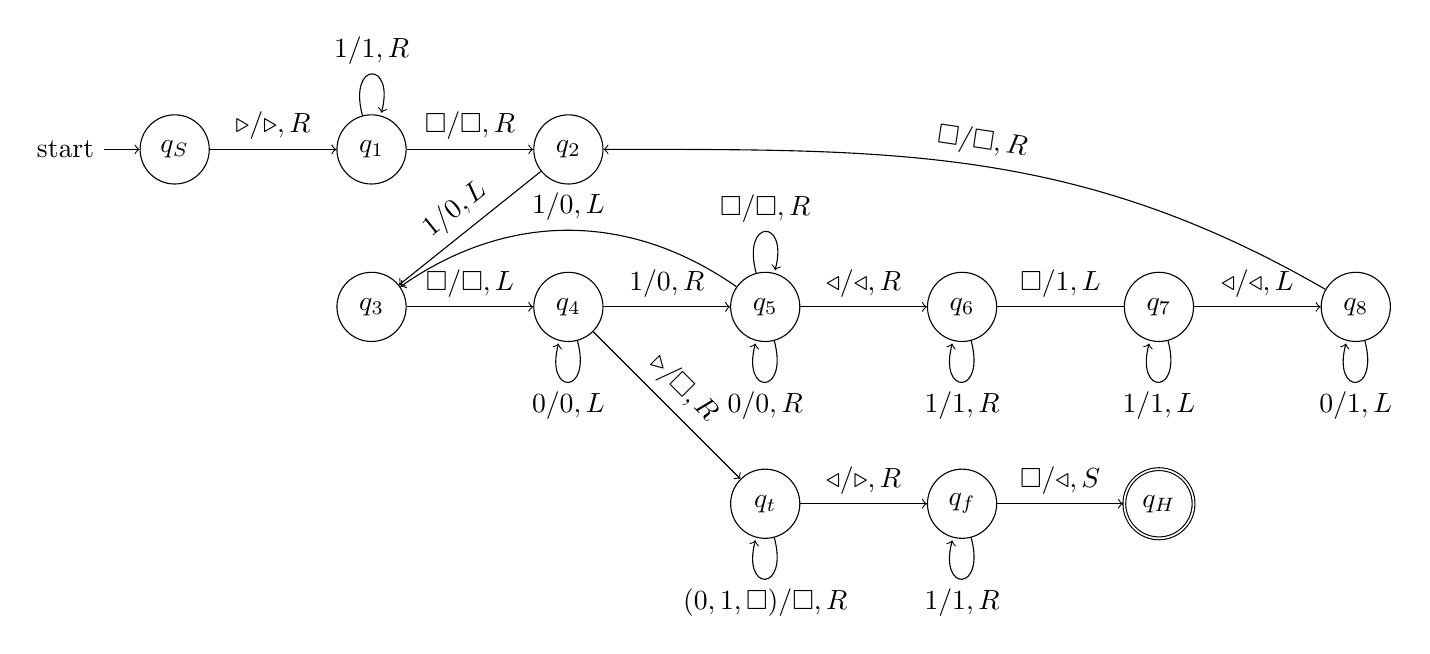
\begin{tikzpicture}[every edge node/.style={font=\scriptsize}]
    \node[initial,state] (v1) at (-1.5,-0.5) {$q_S$};
    \node[state] (v2) at (1,-0.5) {$q_1$};
    \draw[->] (v2) edge[loop above] node {$1\slash 1,R$} (v2);
    \draw[->]  (v1) edge node[above] {$\triangleright\slash \triangleright,R$} (v2);
    \node[state] (v3) at (3.5,-0.5) {$q_2$};
    \draw[->]  (v2) edge node[above] {$\square\slash \square,R$} (v3);
    \node [state] (v4) at (1,-2.5) {$q_3$};
    \node [state] (v5) at (3.5,-2.5) {$q_4$};
    \draw[->]  (v3) edge node[sloped,above] {$1\slash 0,L$} (v4);
    \draw[->]  (v4) edge node[above] {$\square\slash \square,L$} (v5);
    \draw[loop below] (v5) edge node {$0\slash 0,L$} (v5);
    \node [state] (v6) at (6,-2.5) {$q_5$};
    \draw [->] (v5) edge node[above] {$1\slash 0,R$} (v6);
    \node [state] (v7) at (6,-5) {$q_t$};
    \draw [->] (v5) edge node[above,sloped] {$\triangleright\slash \square,R$} (v7);
    \draw [loop below] (v6) edge node {$0\slash 0,R$} (v6);
    \draw [loop above] (v6) edge node {$\square\slash \square,R$} (v6);
    \draw [out=145,in=35,->] (v6) edge node[above] {$1\slash 0,L$} (v4);
    \node [state] (v8) at (8.5,-2.5) {$q_6$};
    \draw [->] (v6) edge node[above] {$\triangleleft\slash \triangleleft,R$} (v8);
    \draw [->] (v8) edge[loop below] node {$1\slash 1,R$} (v8);
    \node [state] (v9) at (11,-2.5) {$q_7$};
    \draw  (v8) edge node[above] {$\square\slash 1,L$} (v9);
    \draw [->] (v9) edge[loop below] node {$1\slash 1,L$} (v9);
    \node [state] (v10) at (13.5,-2.5) {$q_8$};
    \draw [->] (v9) edge node[above] {$\triangleleft\slash \triangleleft,L$} (v10);
    \draw  (v10) edge[loop below] node {$0\slash 1,L$} (v10);
    \draw[->,out=150,in=0]  (v10) edge node[sloped,above] {$\square\slash \square,R$} (v3);
    \draw  (v7) edge[loop below] node {$(0,1,\square)\slash \square,R$} (v7);
    \node [state] (v11) at (8.5,-5) {$q_f$};
    \draw[->]  (v7)  edge node[above] {$\triangleleft\slash \triangleright,R$} (v11);
    \draw  (v11) edge[loop below] node {$1\slash 1,R$} (v11);
    \node [accepting,state] (v12) at (11,-5) {$q_H$};
    \draw[->]  (v11) edge node[above] {$\square\slash \triangleleft,S$} (v12);
\end{tikzpicture}
\end{document}